\documentclass{article}
\usepackage{hyperref} 
\usepackage{url}
\usepackage{amscd,amsmath,amsthm,amssymb}
\usepackage{enumerate,varioref}
\usepackage{epsfig}
\usepackage{graphicx}
\usepackage{subfig}
\usepackage{mathtools}
\usepackage{tikz}
\usepackage{algorithmicx}
\usepackage{algorithm}
\usepackage{algpseudocode}
\usepackage{xcolor}
\newtheorem{thm}{Theorem}
\newtheorem{cor}[thm]{Corollary}
\newtheorem{lem}[thm]{Lemma}
\newtheorem{prop}[thm]{Proposition}
\theoremstyle{definition}
\newtheorem{defn}[thm]{Definition}
\theoremstyle{remark}
\newtheorem{ex}[thm]{Example}
\newtheorem*{rem}{Remark}
\DeclareMathOperator\arcosh{arcosh}
\newcommand{\R}{\mathbb{R}}
\newcommand{\Z}{\mathbb{Z}}
\newcommand{\C}{\mathbb{C}}
\newcommand{\Q}{\mathbb{Q}}
\newcommand{\lrbrack}[2]{\lbrack #1 , #2 \rbrack}
\newcommand{\half}{\frac{1}{2}}
\newcommand{\ket}[1]{|#1\rangle}
\newcommand{\bra}[1]{\langle #1 |}
\newcommand{\tc}[1]{\color{blue} \texttt{#1} }
%\newcommand{\ve}{\vec{1}}


\title{Syllabus for ``A Random Walk Through North America" Summer 2022}
\author{Clark Alexander\\ email: \href{mailto:gcalexander1981@gmail.com}{the author}}

\begin{document}
\maketitle

\section{Main Objectives}

We wish to ``solve" the traveling salesman problem for visiting all the states and provinces in the United States, Canada, and Mexico which are in continental North America.  We will also talk about random walks on graphs and how to implement them in multiple computing langauges.

\section{Daily Goals}
\subsection{Before we Meet}
Get Setup with Julia.  Best method is to download Julia 1.7 from the website and we'll be running in either JuPyter notebooks with iJulia, and for the more sophisticated coder, VSCode.  Recently Atom has foregone the development of Juno REPL and VSCode has taken it over.  

\subsection{Monday}
Morning
\begin{itemize}
	\item Basics of Monte Carlo Methods
	\item How to draw a sample from a distribution
	\item Calculating $\pi$
	\item Markov Chains
	\item Predicting weather for the rest of the week
\end{itemize}
Afternoon
\begin{itemize}
	\item Random Walks on Graphs
	\item How to perform a random walk on a graph
\end{itemize}

\subsection{Tuesday}
Morning
\begin{itemize}
	\item The Simulated Annealing Algorithm
	\item Solving a random TSP
\end{itemize}

Afternoon
\begin{itemize}
	\item How to Set up the North America TSP
	\item Taking our first shot at solving the big one
\end{itemize}

\subsection{Wednesday}
Morning
\begin{itemize}
	\item How to get a better solution
	\item solving smaller problems
	\item Competing Models
	\item Coupled Models (Instructor's Own algorithm)
\end{itemize}
Afternoon
\begin{itemize}
	\item Running our solvers
	\item Intro to Quantum Walks on graphs
	\item Starting our presentation for Coffee talks
\end{itemize}

\subsection{Thursday}
Morning
\begin{itemize}
	\item Computing properties of the North America Graph Walk via Monte Carlo Methods
	\item Quantum Walking Through North America
\end{itemize}
Afternoon
\begin{itemize}
	\item Quantum Walking 
	\item Preparing our presentation Saturday
\end{itemize}

\subsection{Friday}
\begin{itemize}
	\item Random Topics
	\item Working on Presentation
\end{itemize}


\section{Monday}
\subsection{Monte Carlo Methods}

A little history to begin.  Monaco is known for a few things. It's one of the world's tiniest countries, the insanely lavish races culminating in the Formula One Grand Prix, and gambling.  As much as I'd like to spend the rest of the week talking about the Grimaldi Family and their breakaway from the Republic of Genoa in the 12$^{th}$ century, and even more I'd love to talk about the history of F1 in Monaco, but this is math and computer science course and so we're going to start with the gambling.  

Monte Carlo is more-or-less a neighborhood in Monaco, but it's really just the casino district.  The world's high rollers and those who live extravagant lifestyles lose obscene immoral amounts of money there.  But the question we should be asking ourselves is why the ``house always wins?."  If you ever go to a casino in the United States ( and most places in Europe) there will be a sign posted about the house's expected payout.  Here in Chicago it's something like 91\%.  That is, for every \$100 wagered the house collects about \$9.  Now there are two questions.
\begin{enumerate}
	\item Can anyone actually win anything?
	\item How do they know the payout so precisely?
\end{enumerate}

The first answer is yes.  And no.  If one is willing to take a few turns at the roulette wheel and one gets a good spin, then one can walk away a happy person.  I once witnessed this with my own mother.  She decided it would be fun to wager \$20 on the roulette wheel.  She bet on a few random numbers she likes.  One of them hit, she collected her winnings, and we went for a nice dinner. (Of course the house got the money back in an overpriced meal plus tips and wages, but that's another story).  So yes, if one is lucky and extremely cautious simultaneously, one can win. However, the house doesn't care about random mothers and grandmothers winning a single turn of the roulette wheel.  In fact, they quite prefer it.  Why is that?

Our second question can best be answered by a set of techniques we call Monte Carlo methods based on techniques the famous casinos used to make sure the house always wins.

Monte Carlo methods in a nutshell are as simple as can be.
Generate a bunch of random guesses, compute the average.  The more guesses you generate, the closer your average is to the true average.  In the case of a casino, roulette and craps have set probabilities.  So we could generate millions of scenarios randomly and calculate what we would pay out and what the house would keep.  In modern times this is feasible on a laptop as we shall soon see.

\subsection{How to Draw a Sample from a Distribution}

For this course we'll mostly be using Julia 1.6+ as our computing language. So we'll talk about drawing from distributions in this way, but we will also give some tips for python and Octave/MatLab.

Let's start with what a probability distribution is. In order to do this we need to step just a couple paces back.  We need to know what a ``random variable" is.  To make things as simple as possible without the highly technical details of $\sigma$-algebras and Borel spaces, etc, We define a random variable as a function, but the outcome is not deterministic, it's ``random."  A probability distribution is another function that determines the structure of the randomness of the outcome.  A couple of well-known example are coin flipping and rolling dice.
If we roll a single ``fair" die we have the outcomes $\{1,2,3,4,5,6\}$ each with probability $1/6$.  So the distribution is called a uniform distribution since each outcome is equally likely.  With two dice we have the outcomes $\{2,3,4,5,6,7,8,9,10,11,12\}$ but the probabilities are not uniform.  They are $\{1/18,1/12,1/9,5/36,1/6,5/36,1/9,1/12,1/18\}$


Some more common distributions we use and will use for this set of notes are the normal distribution and the uniform distribution on and interval. We will also need to draw samples from unnamed distributions, but those arising from experiments which we'll perform.


In Julia we use the packages Distributions and Random.
using Random, Distributions

To draw a random normal variable with mean 0, deviation 1. we type
a = randn()

for an entire vector of 100 random normal variables
vec = randn(100)

\subsubsection{Julia}

\subsubsection{Python}

\subsubsection{Octave}


\subsection{Example: Calculating $\pi$}

Now let's go through a fun example.  Let's calculate the value of $\pi$ using a Monte Carlo simulation.  Our approach will be to simply pick random points in the unit square and see how many have length less than one.
Put simply, we'll count how many land inside the quarter circle versus how many random points we've chosen.


The code is easy \ref{MCpi}
\begin{algorithm}
	\caption{Monte Carlo $\pi$ calculation}
	\label{MCpi}
	\begin{algorithmic}[1]
		\Procedure{Calculate $\pi$}{numberTrials}
		\State points = rand(numberTrials,2)
		\State count = 0
		\For {$p = 1:$numberTrials}
		\If {norm(points[p,:]) $< 1$}
		\State count $+= 1$
		\EndIf
		\EndFor
		\EndProcedure
	\end{algorithmic}	
\end{algorithm}   

Now we compute count/numTrials which is approximately $\pi/4$ so we have
\[
 \pi \approx 4*\text{count}/\text{numTrials} 
\]

The more samples we take, the closer we are.  What happens when we combine the whole class's answers collectively?

\subsection{Markov Chains}

A Markov chain is a sequence of events where each subsequent event depends on the previous one.  A little more precisely when we have a sequence $\{x_n\}_{n=0}^{N}$ the probability that $x_{N+1}$ will produce a certain value is conditioned on the value of $X_N$
\[
Pr(x_{N+1} =  \alpha | x_N = \beta)
\]

If we follow this inductively, this gives us a chain of events.
\[
Pr(x_{N+1} =  \alpha | x_N = \beta, x_{N-1} = \gamma, ... x_0 = \zeta)
\]

The secret is that the events of two previous points in the sequence are ``baked in."

There are two relatively distinct types of Markov Chains, discrete and continuous.  For the moment we'll focus on the discrete Markov chain.  Let's take an example.  Let's say we've been observing the weather daily for the last year and we wrote down only the whether or not we had precipitation.
At the end of year we have 365 observations 75 of which had precipitation; which gives us 290 days without.  Naively we say the probability of rain is 70/365 for the next day.  However, if tomorrow it rains the next day's probability will be 71/366 and if not 70/366.  However, weather is a little more complicated than counting raw numbers.  We recognize, from having lived, that two days of sun in a row are more likely than two days of rain.  But a day of rain is likely to follow another rainy day.

So for our 365 days we have 364 ``next day" items to consider.  Now look at this matrix
\[
\begin{tabular}{l | c | c}
today $\backslash$ tomorrow & precipitation & none \\
\hline
precipitation    &    35         &   40 \\
\hline
none             &    40         &   250
\end{tabular}
\]  

This gives us a better picture of what to expect tomorrow.  That is to say, if today is rainy, we have a likelihood 35/75 to see more precipitation tomorrow.  If, on the other hand, it's nice and sunny today, our chances of seeing rain have been substantially reduced.  This gives us a prime example of a discrete Markov chain.

More formally, if we have a probability start (a vector which sums to 1) the next state is determined by a transition matrix which is what we have constructed above.
\[
p_{n+1} = M p_{n}
\]

Our example is starting in the state $p_0 = \begin{bmatrix}
0\\1
\end{bmatrix}$ (no precipitation)

\[
p_1 = \begin{bmatrix} 0.47 & 0.13\\
0.53 & 0.87\end{bmatrix} \begin{bmatrix}
0\\1
\end{bmatrix} = \begin{bmatrix}
0.13 \\ 0.87
\end{bmatrix}
\]

However two days from now we have
\[
p_2 = M^2 p_0 = \begin{bmatrix}
0.175 \\ 0.825
\end{bmatrix}
\]

This tells us, it's slightly more likely to rain in two days than it is tomorrow.  In weather forecasting we will collect many, many, many more weather types, in addition to precipitation and not, we collect temperatures, barometric pressure, inches of precipitation, etc. So instead of a $2\times 2$ matrix, we'll have a $100000\times 100000$ matrix.  In order to predict the rest of the week's weather we consider the transition matrix to the 5$^{th}$ power.


\begin{rem}
	The continuous Markov chains follow exactly the form you'd expect with the difference replaced by a derivative
	\[
	\frac{dp}{dt} = M p(t)
	\]
	We'll see this show up in a big way later in our course.
\end{rem}


\subsection{Predicting this Week's Weather}

One this that is important in weather prediction is that we're beginning with frequentist statistics and from them we make Bayesian predictions.  The transition matrices are based purely on observation.  

So let's give this a try.  Consider the following matrix:
\[
M = something
\]

Let's get a quick prediction for tomorrow, Wednesday, Thursday, Friday, and Saturday.

We will set today's vector appropriately and call it $p_0$. Notice this should be a measured data point.  So we again use the frequentist statistics as a starting point.  Let's run a million simulations (as a class) and see what we come up with.

\subsection{Random Walks on Graphs}

Before we go to a general graph let's start with an easy random walk.
Let's imagine we're on a side walk with roughly square sections.  Instead of moving along linearly, let's walk along randomly according to a coin flip.  Let's flip a coin and if it's heads we step forward, tails we step back.  My question to you is, after 100 flips where are we?  The answer is, we don't know, but we're roughly close to where we started.  In fact with high likelihood we're within 10 $\sqrt{100}$ steps of where we started. 
On a graph, we may have a slightly more complicated relationship.

Consider the following graph

\[
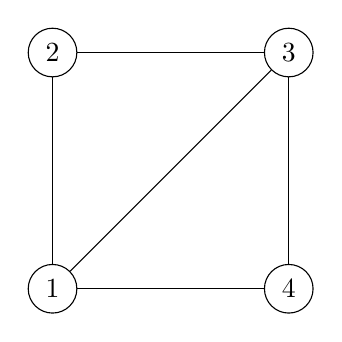
\begin{tikzpicture}
\node[circle,draw] (1) at (0,0){1};
\node[circle,draw] (2) at (0,3){2};
\node[circle,draw] (3) at (3,3){3};
\node[circle,draw] (4) at (3,0){4};
\foreach \from/\to in {1/2,1/3,2/3,3/4, 1/4}
\draw (\from) -- (\to);
\end{tikzpicture}
\]

If we start at vertex 1, we have 3 possibilities.  So with probability 1/3 we move to each of the vertices 2,3,4.  If we move to vertex 2, then we only have two possibilities.

For historical reasons, we tend to think of the random walk as a row vector as opposed to the more common (in textbooks) column vector.  So our equation becomes
\[
p_{n+1} = p_n W
\]

In this case $W$ is the matrix which encodes both the graph structure and the probabilities.

\[
W = D^{-1}A = \begin{bmatrix}
3 & 0 & 0 & 0\\
0 & 2 & 0 & 0\\
0 & 0 & 2 & 0\\
0 & 0 & 0 & 2
\end{bmatrix} 
\begin{bmatrix}
0 & 1 & 1 & 1\\
1 & 0 & 1 & 0\\
1 & 1 & 0 & 1\\
1 & 0 & 1 & 0
\end{bmatrix} = 
\begin{bmatrix}
0 & 1/3 & 1/3 & 1/3\\
1/2 & 0 & 1/2 & 0\\
1/3 & 1/3 & 0 & 1/3\\
1/2 & 0 & 1/2 & 0
\end{bmatrix}
\]

The matrix $D$ is the \emph{degree} matrix which encodes the degree of each vertex.  In this way we can encode the probabilities of moving to another vertex.  The matrix $A$ is the \emph{adjacency} matrix which encodes which vertices are connected via a single edge.   



\subsection{How to Perform a Random Walk on a Graph}

Now we want to perform a random walk on an actual graph.  Let's keep with our 4 vertex graph from above.  In order to perform a random walk, we need a starting point. Let's start at vertex 1.
\[
p_0 = [1, 0, 0, 0]
\]

Now we compute $p_1$ and draw the next vertex from the distribution $[0, 1/3, 1/3, 1/3]$.
This gives us vertex two.  So our walk is $v1,v2$ now we choose from 1 and 3 with probability $1/2$. We continue this as long as we want.

I tried this for 5 steps and got $v_1,v_2,v_1,v_4,v_3,v_1$.

\subsubsection{Some Interesting Statistics about Random Walks on Graphs}

Here we present some definitions, and we'll leave the harder exercises for your later classes.
\begin{defn}
	The \emph{hitting time} $H(u,v)$ for a random walk from vertex $u$ to vertex $v$ is the minimum expected time $t$ so that the value of the walk at time $t$ is $v$ where the value at time $0$ is $u$. Formally
	\[
	H(u,v) = \mathbb{E}\left[\{t\in \mathbb{N}| X_t=v\} | X_0 = u\right]
	\]
\end{defn}

\begin{defn}
	The \emph{cover time} of a graph from a vertex $u$ is the minimum amount of expected time in which a random walk visits every vertex in a (connected) graph.  The cover time of a graph is the maximum of all the cover times of individual vertices.
\end{defn}

We'll try to get a hold on these via Monte Carlo methods for a big graph later on. Probably Thursday.

The main thing I wanted to talk about in this particular sub section is the stationary vector and how we get there.
For historical reasons we call this vector $\pi$.  It's defined by
\[
\pi = \pi W
\]
where $W$ is the walking matrix we've defined above.  You'll notice from the definition that this is the eigenvector with eigenvalue 1 for the matrix $W$.  We know that such a vector exists since we have defined our matrix $W$ the have every row sum to 1.  In fact, we know this is the largest eigenvalue because we've normalized every row, so that the resulting vectors are probability distributions.

If you've every worked with an algorithm computing the largest eigenvalue you'll recognize:
\[
\pi = \lim_{n\rightarrow \infty} p_n = \lim_{n\rightarrow \infty} p_0 W^n
\]

The interesting thing (to me) is that we don't have to go to $\infty$.  
\begin{thm}
	Given a connected graph $G$ and associated walking matrix $W$ and an initial random walk vector $p_0$ 
	\[
	\| \pi - p_0 W^t\| \in O(\lambda_2^t)
	\]
	Where $\lambda_2$ is the second largest (absolute) eigenvalue of $W$.  
	
\end{thm}

The difference between $\lambda_1 = 1$ and $\lambda_2$ is called the \emph{spectral gap}. The larger the spectral gap, the fewer steps to get to the stationary vector.  For graphs in which the spectral gap is particularly large, these graphs are called expander graphs and in extreme cases are called \emph{Ramanujan} graphs.  Generally, we expect Ramanujan graphs to be regular graphs, but we can still calculate the spectral gap on a normal graph, especially for the purposes of finding how long it will take to reach the vector $\pi$



\section{Tuesday}

Today we're going to turn our knowledge gained yesterday into an ability to optimize difficult problems.  The goal, of course, is to allow randomness to do a lot of the hard work for us and not go through the brute force calculations.  In particular when we have a potential solution space which grows exponentially or faster, we cannot check all the possibilities.  We'll run out of time.  Just some quick ``back-of-the-envelope" calculations show us how long it would take to achieve the exact solution.  Let's start with two quick examples.
\subsubsection{Choosing a Stock Portfolio}
A bunch of empirical studies (hidden Monte Carlo methods in action) show us that a good amount of stocks to invest in at a time is 20.  On the Bolsa de Valores there are 144 stocks listed.  How many portfolios of 20 stocks are there?
\[
\binom{144}{20} \approx 1.51 \times 10^{24}
\]

That's a lot!  Consider a modern laptop can operate at roughly 3 GHz ($3\times 10^9$) this means it would take us
$4\times 10^{14}$ seconds to calculate each portfolio if the individual calculations only cost us one flop.  That's about 16 million years.  I guarantee your laptop won't last that long.  So this is obviously not feasible.

If you go to the Nasdaq where there are more than 3000 stocks available, well, that becomes infinite (to first approximation).  There must be a better way.

\subsubsection{The Traveling Salesman Prblem}
This is one of the classics in computing theory.  We want to start our journey at ``home" and visit some fixed number of sites (usually cities or businesses) and return home having traveled the shortest distance.  
This grows as $n!$ where $n$ is the number of places we have to visit (including home).  For 19 additional cities this is already $2.4\times10^{18}$ possibilities.  We're going to try this week to ``solve" a problem with 95 cities which lands us on
\[
95! \approx 1.03 \times 10^{148}
\]

No supercomputer or cluster of supercomputers nor quantum computer no nothing, can handle that size problem.


\subsection{The Simulated Annealing Algorithm}

Let's talk about annealing first.  Yes, metallurgy.  What is annealing in the metallurgical sense?  The idea is that a raw piece of metal which we get by mining or sifting through dirt or picking out of a riverbed has a lot of impurities. To really make a good point about the impurities of metals consider this fun story.

It is said that the king of Siam (now Thailand) in the early 1800s was the richest man in the world.  During a meeting with Napolean Bonaparte this wealth was on display.  At a formal dinner, Napolean's men ate with silver utensils, while Napolean himself ate with gold utensils.  The king of Siam, however, ate with aluminum utensils.  Now you're thinking, what the ****!? Aluminum is super cheap!  Not in the early 1800s it wasn't!  Aluminum has so many impurities in it that finding a sample pure enough from which to make utensils made aluminum the most valuable metal in the world at that time.  

Now let's come to the present.  Aluminum is super cheap, and that's because it turns out, it's very easy to remove impurities by electrolysis.  The older technique of annealing became prevalent in sword making.  Annealing is the process of taking a metal with impurities and heating it up to some extreme temperature where all the impurities burn off and as it cools, one can bend and shape the new metal into a new shape which will be much stronger.  This is what happens in the process of making iron into steel. In sword making, if one hammers out a piece of iron into a sword, then heats it up to extreme temperatures and quickly cools it (while emblazening the master maker's mark) we get extraordinary swords.  One can also see this technique at work in high quality kitchen knoves these days.  

Now, our goal is to turn this optimization process of metals into an optimization process for combinatorial problems.  As in basic Monte Carlo methods, we let nature guide us, rather than trying to be too clever at the beginning.  So simulated annealing involves a temperature parameter which we start ``hot" and reduce to ``freezing" at some rate.  There are so many ways to do this, but the basic process is the following:
\begin{enumerate}
	\item Guess a solution
	\item Using the first solution guess a second solution, called a neighbor (This is a Markov Chain Monte Carlo step)
	\item score both solutions
	\item if the ``new solution" is better than the ``old solution" accept it immediately and make this the``old solution"
	\item If the ``new solution" is worse, we still might accept it, and that is based on how much worse it is, and the temperature.  
	\item Lower the temperature
	\item Repeat until ``freezing"
\end{enumerate}

Now you're looking at this and you got stuck at step 5, and probably blurted out some expletive and said, this guy is totally mad, why!? NO! STOP! That's not how to find an optimal solution!  But dear friends, this is a highly effective method and let me explain why.

If we only use neighbors to find better solutions, this amounts to a simple guess and check method, and is likely to get us stuck in a local minimum.  Here's a good analogy.  We want to find the highest peak in a mountain range, but we don't know where to start.  So we climb the hill closest to our house.  We never accept going down hill.  Once we reach the top of our local hill, we look around and see any direction we step is downward.  Thus we have reached the highest peak, right?  Obviously no.  We look to the next hill over and realize if we had started there, we would have landed at a higher elevation.  So what went wrong?  Our strategy was too rigid.  Since our solution has so many possibilities, the likelihood that we started in the ``right place" for a strict uphill climb to the top is very low.  Thus we allow ourselves to jump around to neighoring hills once in a while to give ourselves a better shot at reaching the highest peak.

In simulated annealing, we generally look for the minimum, but this can easily be made into a maximization problem by looking for the lowest value of $-f$ and wiping away to negative sign at the end.


So here's our pseudo-code
\begin{algorithm}
	\caption{Simulated Annealing}
	\label{SA}
	\begin{algorithmic}[1]
		\Procedure{Minimize ``score"}{$x_0$, $T_0$, $T_f$, trials\_per\_degree}
		\State oldSolution = $x_0$
		\State oldScore = score($x_0$)
		\State bestolution = neighbor($x_0$)
		\State bestScore = score($x_0)$
		\State $T = T_0$
		\While{$T > T_f$}
		\For{k = 1:trials\_per\_degree}
		\State newSolution = neighbor(oldSolution)
		\State newScore = score(newSolution)
	    \If{newScore $<$ bestScore}
	    \State bestScore = newScore
	    \EndIf
	    \If {acceptanceProbability(oldScore, newScore, T) $> U(0,1)$}
	    \State newSolution = oldSolution
	    \State newScore = oldScore
	    \EndIf
	    \EndFor
	    \State Lower $T$
	    \EndWhile
		\EndProcedure
	\end{algorithmic}	
\end{algorithm}   


You can see here there are several auxiliary functions we need to define, and that's the beauty of simulated annealing.  It can be tuned to any kind of problem.  We need to define how to score a solution, how to pick a neightbor, how much tolerance we have for selecting a worse solution, and at what rate we wish to lower the temperature.  These particulars must be tuned for each problem, but luckily I have enough practice runs at this to help guide you in picking these functions.


\subsection{Solving a Random Traveling Salesman Problem}

Now let's take this toy out for a spin.  We're going to minimize the route we need to take around the unit square and visit 50 different points along the way.  First we'll generate our points randomly, and then I'll provide a set of pre-selected points.  Let's see who can get a really small solution.

Some suggestions here. For the time being, distance will be the standard Euclidean distance in 2D.
\[
d(x,y) = \|x-y\| = \sqrt{(x_1-y_1)^2 + (x_2-y_2)^2}
\]]

The score will be the sum of all distances traveled including returning home.
So we'll have
\[
 \text{score} = \sum_{n=0}^{50} d(x_n,x_{n+1}) \text{with} x_0 = x_{50}
\]

The acceptance probability is fairly common
\[
\exp((oldScore - newScore)/T)
\]

Notice two things here.  If the new score is smaller, the probability is automatically greater than 1, and so will be immediately accepted.  Second, as the temperature cools, we get more strict about how much worse the solution is before we accept it.
For example if $T = 100$ and new score $=2$ with old score $=1$
\[
\exp((1-2)/100)) \approx 0.99
\]

So we're very likely to accept that.  Later when our temperature gets down to say $T = 0.1$
\[
\exp(1-2)/(0.1)  \approx 1\times 10^{-10} \approx 0
\]

We're extremely unlikely to allow this to happen.


In the department of lowering temperature, there are two common ways: linear and geometric.  I generally prefer the geometric
\[
T *= \alpha
\]

where $\alpha < 1$ but reasonably close.  Something like $0.95$.  There are not set rules on this.  The second common way is just decrementing by some fixed linear amount

\[
T -= 0.01
\]


However, there are lots of ways to do this, in fact, one can pick any montonically decreasing function, so that the temperature can slow down at points to allow more explanation and speed up when solutions get better. For example, consider that we want to slow down our temperature around $0.4$  We can pick a sequence of temperatures as follows

\begin{algorithm}
	\caption{Custom Temperature Decrement for Simulated Annealing}
	\label{Custom Temperature}
	\begin{algorithmic}[1]
		\Procedure{Slow at $T=\beta$}{numTemperatures}
		\State Section1 = $(\beta + 0.001) + (1 - 0.001 - \beta)*rand(n/3)$
		\State Section2 = $(\beta - 0.001) + (0.002)*rand(n/3)$
		\State Section3 = $(\beta - 0.001)*rand(n/3)$
		\State Temperatures = sort([Section1;Section2;Section3], reverse = true)
		\EndProcedure
	\end{algorithmic}	
\end{algorithm}   

In our annealing algorithm we replace the while loop with a for loop $T$ in Temperatures.


The final piece, and potentially the most crucial is selecting a ``neighboring" solution from the current one.  In the traveling salesman problem, if we pick completely randomly, and plot our path it looks like a big tangle.  A ``solved" problem has a few ``obvious" characteristics; namely, no loops and no crossings.  If you ask a random person to draw you a solution, they will use some sort of heuristics like that.  So our goal as a machine teacher is to tell the computer how to ``untangle" the mess.  Again, there are multiple suggestions, but the simplest (for a small problem) is pick a section at random and reverse the order in which it is traversed.  This is equivalent to telling the computer to try to untangle a section at a time.  It also allows us to see why we might accept a slightly worse answer if there are a lot of tangles still remaining.

One can pick any number of variations on that theme.  Unravel two separate sections at a time, switch two points only, move through a cycle of 3,4,5,6,7,etc points.  Randomly exchange ten points, switch two adjacent points, etc.  


\subsection{How to Set up the North America TSP}

For our main project this week we're going to thoroughly examine the graph of (connected) North America.  That is, 13 Canadian Provinces, 49 states and Washington D.C. in America, and 31 states and the Federal District of Mexico which brings us to 95.  Quick aside, while Alaska is not connected to the other 48 states, it is connected to Canada, so we're including it here as part of the connected component.  Additionaly, Prince Edward Island and Nova Scotia in Canada are not connected by a physical land border, but they are connected by bridges, so we include them here as well, since they are lovely places, and we don't want to cheat and give ourselves any advantages.  We really want to travel through North America.

We will have two sets of distances.  The first is the flying distance between capital cities of these regions. That will be computed using Earth's great circle calculation (and taking into account that Earth is squished a little).  I'll provide those calculations for you.  That will be a $95\times 95$ matrix.  Additionally, we'll use driving miles which I'll also provide, but looked up through google maps.

Our task is to start in Guadalajara and traverse the other 94 cities and return here in as little distance as possible.  This calculation in this case will be done by simple look-ups rather than calculating the Euclidean distance for each pair.

\subsection{Taking Our First Shot at the Big One}

Now that we have set up our distance calculations and our goal of minimizing said distance, let's take a shot at solving both of these problems.  What I want is for people to split up into teams of 3 and try out different strategies for picking neighbors.  Let's see who comes up with the shortest distance by day's end!



\section{Wednesday}
\subsection{How to get a better Solution}
\subsection{Competing Algorithms}
\subsection{Coupled Models}
\subsection{Intro to Quantum Walks on Graphs}

\section{Thursday}
\subsection{Properties of the North America Graph via Monte Carlo}
\subsection{A Quantum Walk Through North America}

\end{document}